%!TEX root = ../../../main.tex

\subsection{Requirements}

We can arrange the defined requirements using the \acrfull{furps} model \parencite{furps}.

\subsubsection{Functionality}

These constraints define the capability, reusability and security of a given project or application. In the scope of this project we can define the following requirements (see figure \ref{fig:usecases}:

\begin{itemize}
	\item A privileged developer can integrate new \acrshort{hpo} algorithms into the framework
	\item A developer can define all necessary information to allow the optimization pipeline to run (hyper parameter definitions, objective function instantiation, algorithm selection, etc.)
	\item A developer can obtain information during and at the end of the optimization process regarding said process
	\item A developer can run the optimization pipeline.
\end{itemize}

\begin{figure}[hb]
\centering
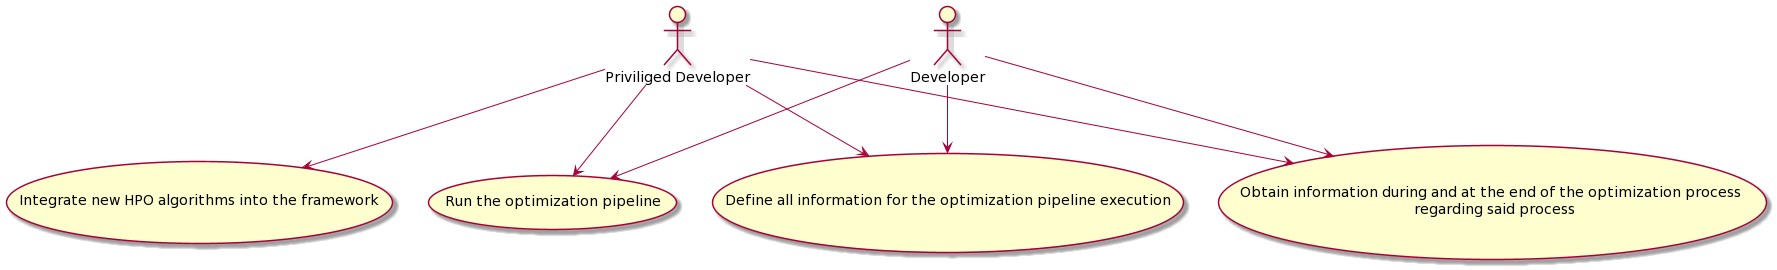
\includegraphics[width = \textwidth]{images/domain_model.png}
\label{fig:usecases}
\caption{Defined Use Cases}
\end{figure}


Here we define a privileged developer as a developer who is connected to the development of the framework.

\subsubsection{Usability}

These constraints define how the interaction between a user and the program occurs, as well as, for example, the available documentation. In the scope of this project we can define the following requirements:

\begin{itemize}
	\item There should be comprehensive documentation on how the system functions and how a user interacts with it
	\item There should be pre-existing examples of usage of the system.
\end{itemize}

\subsubsection{Reliability}

These constraints define important factors such as the availability and robustness of the system, as well as its accuracy and stability. In the scope of this project we can define the following requirements:

\begin{itemize}
	\item The system should be able to recover from external failures (eg.\ issues with CAM2\textsuperscript{\textregistered})
	\item The system should be able to save its state in order to allow for interruptions in the execution.
\end{itemize}

\subsubsection{Performance}

These constraints define what the expected performance of a given application is, using metrics such as speed, efficiency, resources consumption and others. In the scope of this project we can define the following requirements:

\begin{itemize}
	\item The software should be faster than the CAM2\textsuperscript{\textregistered}'s endpoints it accesses
	\item The software should be efficient in such a way that it does not interfere with the CAM2\textsuperscript{\textregistered} software
	\item The system should consume as little resources as possible, allowing for it to be run directly in the developer's issued laptop, without interfering with other programs.
\end{itemize}

\subsubsection{Supportability}

These constraints define how easily the developed project is supported and used by others. To do this, we can define goals regarding testability, modifiability, installability and others. In the scope of this project we can define the following requirements:

\begin{itemize}
	\item The developed code should include meaningful testing, insuring the correct operation of the software
	\item The developed system should allow for extending its usage to new algorithms and optimizable functions
	\item The developer should be able to define their preferred configuration when executing the software
	\item The software should be installable in any of \faro's issued laptop easily.
\end{itemize}

\subsubsection{Design Constraints}

These constraints define the design of a system and may include programming languages, software processes, tool usage and others. In the scope of this project we can define the following requirements:

\begin{itemize}
	\item The developed application must be implemented in Python.
\end{itemize}

\subsubsection{Implementation Constraints} 

These constraints define how the project is developed and may include required standards, resources limitations and others. In the scope of this project we can define the following requirements:

\begin{itemize}
	\item The developed application must executed with minimal resource allocation (with regards to CPU usage and RAM allocation)
	\item The developed application must be able to execute in a Windows environment.
\end{itemize}

\subsubsection{Interface Constraints} 

These constraints define how the communication between various components of the project is executed. Within the scope of this project, we can define constraints based on the communication between the CAM2\textsuperscript{\textregistered} software and the developed project:

\begin{itemize}
	\item The optimization pipeline must allow communication with the CAM2\textsuperscript{\textregistered} integrated web server
	\item Said communication must be executed through \acrfull{http}, using pre existing endpoints.
\end{itemize}

\subsubsection{Physical Constraints}

These constraints define the physical limitations for the system. Such constraints can be material, shape or weight specifications when referring to a hardware project but also refer to, for example, network requirements or topology when referring to software projects. In the scope of this project we can define the following requirements:

\begin{itemize}
	\item The developed system should be executed in the same network as the CAM2\textsuperscript{\textregistered} integrated web server.
\end{itemize}
